\documentclass{article}

\title{	
	\normalfont\normalsize 
	\rule{\linewidth}{0.5pt}\\ % Thin top horizontal rule
	\vspace{14pt} % Whitespace
	{\LARGE MATH401 Assignment 1 \\ % The assignment title
    \large \textit{} \\}
	\vspace{6pt} % Whitespace
	\rule{\linewidth}{1pt}\\ % Thick bottom horizontal rule
}

\author{Elliott Hughes}
\date{\normalsize\today}
\usepackage{tikz}
\usetikzlibrary{arrows,automata}
\usetikzlibrary{positioning}
\usetikzlibrary{arrows.meta,positioning}
\usepackage{mdframed}
\usepackage{amsmath}
\usepackage{amssymb}
\usepackage{graphicx}
\graphicspath{ {./Images/Assignment_1/} }
\usepackage{commath}
\usepackage{textcomp}
\usepackage{gensymb}
\usepackage{float}
\usepackage{hyperref}
\usepackage[margin=1in]{geometry}
\usepackage{caption}
\usepackage{subcaption}
\usepackage{sectsty}
\usepackage{titlesec}
\usepackage[backend=biber, style=ieee]{biblatex}
\addbibresource{Assignment_1.bib}
\setlength{\parskip}{-0.2cm}

\begin{document}

\maketitle

\section*{Q15}
\subsection*{(a)}
Rounding to four decimal places, the first six points in the forward orbit of $a_0 = 0.15$ are 
$\{0.4890,\,0.9583,$ $0.1533,\,0.4978,\,0.9587,\,0.1517\}$. We now wish to show that the interval 
$[0.15,0.1533]$ is mapped inside itself by $f^3$. To do this, it is necessary to show that the 
end-points of this interval are mapped inside $[0.15,0.1533]$ by $f^3$ and that $f^3$ is locally 
monotonic on this interval (as if $f^3$ is not monotonic then this could lead to points inside this 
interval being mapped above or below the relevant endpoints).

\paragraph{}
From our above analysis of the first six points in the forward orbit of $a_0$ we have already shown 
that $f^3(a_0) = 0.1533$ and that $f^3(0.1533) = 0.1517$. The first derivative of the function 
was obtained computationally and it was verified that any zeros of the first derivative of $f^3$ 
lay outside the interval of interest. The closest zero is at $0.1541$ which is clearly outside 
the domain. The first derivative of $f^3$ at $a_0$ is $-0.7988$, so it follows that the 
function must be decreasing across $[0.15,0.1533]$ and thus will map this interval inside itself 
(see \autoref{fig:f^3_slope} below for a sketch of $f^3$ across the domain of interest).

\begin{figure}[H]
    \centering
    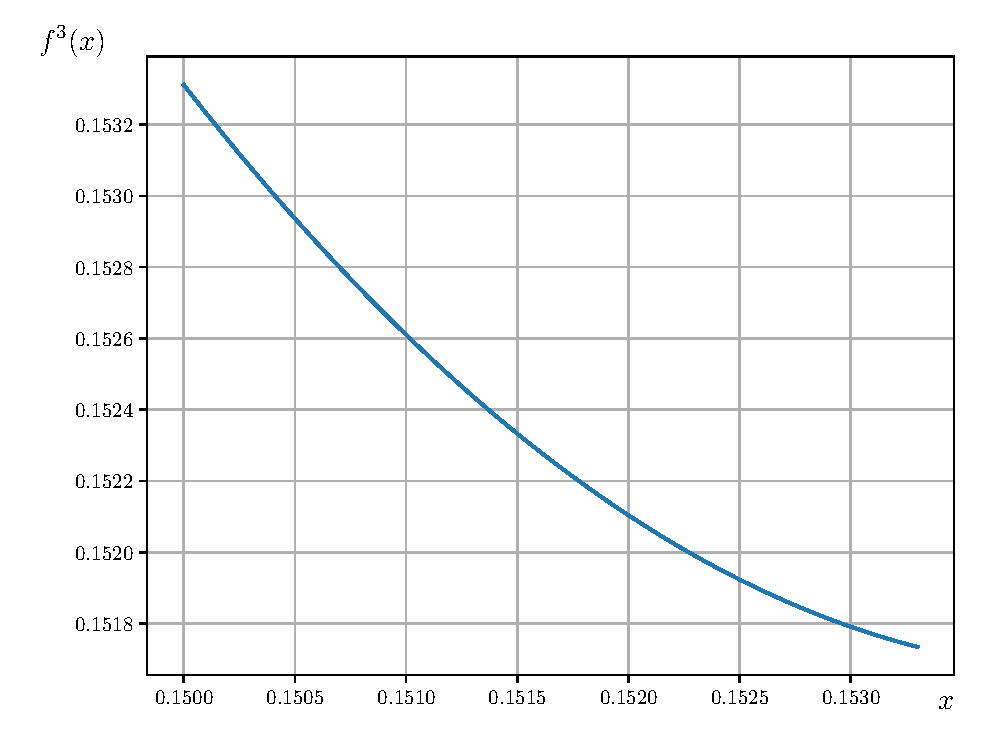
\includegraphics[scale = 0.6]{Figure_1.eps}
	\caption{$f^3$ on the domain of interest.}
    \label{fig:f^3_slope}
\end{figure}

\subsection*{(b)}
Since $f^3$ is a polynomial it is continuous, so we can directly apply the Lemma presented on 
page 15 of the notes and consequently obtain that there exists a fixed point in the interval 
$[0.15,0.1533] \subset [0,1]$ as $f^3([0.15,0.1533]) \subset [0.15,0.1533]$. A point which is 
fixed under $f^3$ must either be a fixed point of period one or a period three point. However, 
we know from previous work that the only fixed points of $f$ are at 0 and at $(3.385-1)/3.835 = 0.7392$ 
neither of which lie in this interval. Consequently there must be a period three point that lies 
within this interval.

\subsection*{(c)}
Repeating our strategy from part (a), we wish to show that $|(f^3)'|$ is less than 0.8 at the endpoints 
of this interval and that $(f^3)'$ is monotonic on this interval. Computing $(f^3)'$ we obtain that  
$(f^3)'(0.15) = -0.7988$ and that $(f^3)'(0.1533) = -0.1572$ so if $(f^3)'$ is monotonically 
increasing on this interval then $|(f^3)'| < 0.8$ on this interval. It can be shown that the second derivative has no zeros on the range of interest 
(the closest zeros occur at $0.0826$ and at $0.2281$ respectively). Therefore $|(f^3)'| < 0.8$ 
as required (see \autoref{fig:f^3'_slope} for a sketch of $(f^3)'$ on the domain of interest).

\begin{figure}[H]
    \centering
    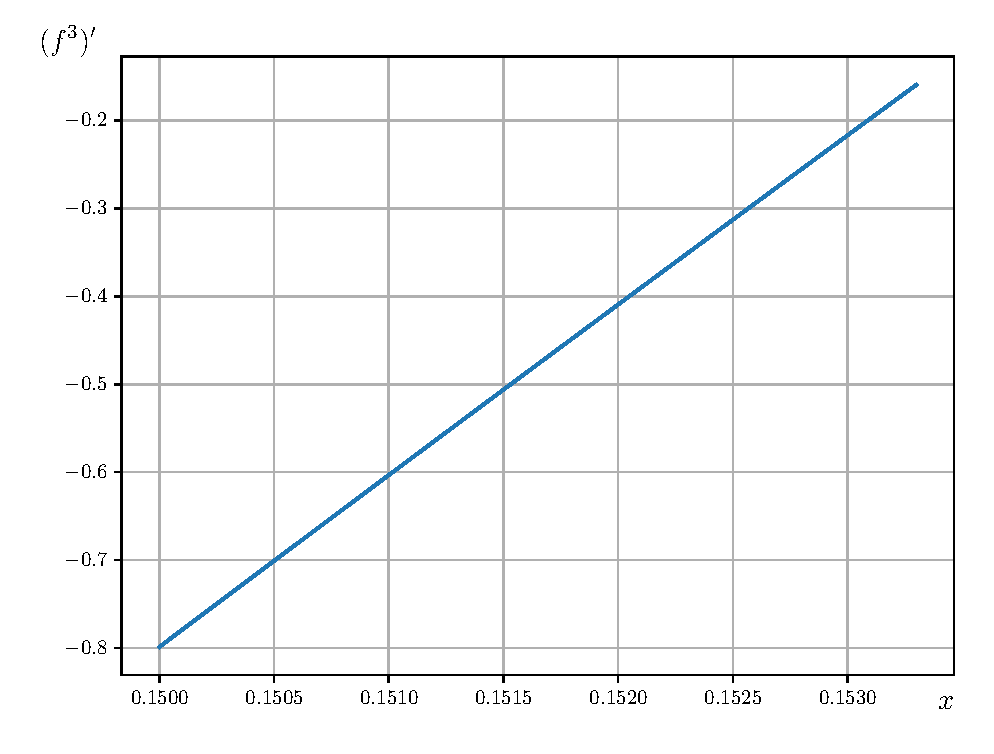
\includegraphics[scale = 0.6]{Figure_2.eps}
	\caption{$(f^3)'$ on the domain of interest.}
    \label{fig:f^3'_slope}
\end{figure}

\paragraph{}
Since $|(f^3)'| < 1$ in this interval, this suggests that at the period-3 point inside this 
interval $|(f^3)'| < 1$ and consequently that this point is attracting under $f^3$. This implies 
that this period-3 orbit must be attracting under $f$.

\subsection*{(d)}
By directly computing the first 100 orbits of $a_0$, we obtain some numerical results that support our 
statement that this period-3 point is attracting. Under repeated iterations, $a_0$ appears to 
approach a period-3 orbit (see attached histogram).

\begin{figure}[H]
    \centering
    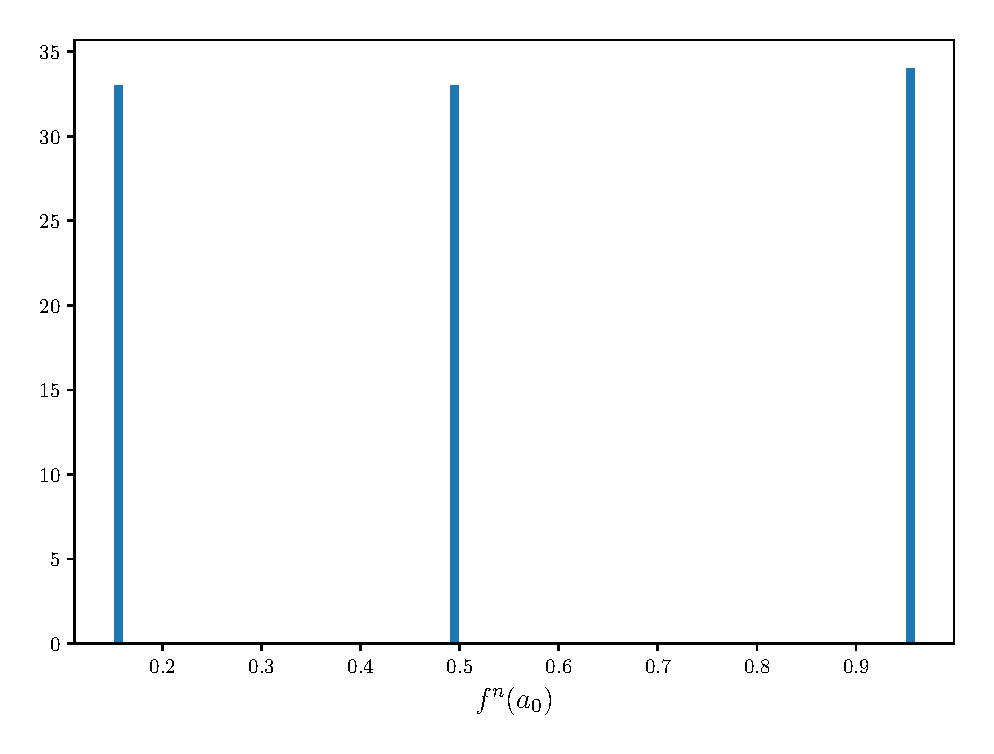
\includegraphics[scale = 0.6]{Figure_3.eps}
	\caption{Histogram of the values of first 100 points in the orbit of $\mathcal{O}(a_0)$.}
    \label{fig:f_histogram}
\end{figure}

\paragraph{}
Starting from $a_0 = 0.15$, it is clear that the first 100 points in the orbit are confined into 
three small regions of the domain of $f$ and points are approximately evenly distributed between these 
three regions. This provides strong, although not definitive, evidence in support of the attracting 
period three orbit we found in parts (a-c).

\section*{Q16}
Before we can analyze behavior around this attracting period-3 window, it is first necessary to 
locate this window and choose appropriate parameter values. From Q15, we know an attracting period-3 
orbit must exist near 3.835, so by plotting the bifurcation diagram around 3.8 it may be possible 
to see the approximate boundaries of this window (\autoref{fig:bifn_logistic}).

\begin{figure}[H]
    \centering
    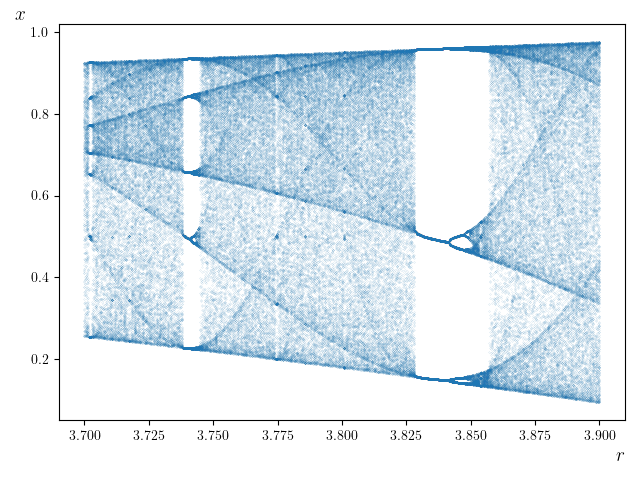
\includegraphics[scale = 0.7]{Figure_4.png}
	\caption{Numerically obtained bifurcation diagram of the logistic map around 3.8 (only stable 
    points are shown).}
    \label{fig:bifn_logistic}
\end{figure}

\paragraph{}
The above diagram suggests that the window where an attracting period 3 orbit exists (e.g. the 
region where there are three distinct branches apparent in the bifurcation diagram) ranges from 
about 3.83 to 3.86. Therefore, we select as our parameter values of interest the set $\{3.7, 3.835, 3.86\}$ 
(while the smallest parameter value could be increased, choosing a smaller value makes the change 
in the dynamics clearer). 
Next, for each of these parameter values we plot $f^3$, $f$ and the line $x_{n+1} = x_n$. This enables us 
to straightforwardly identify the relative positions of fixed points of period 3 and those of 
period 1 (\autoref{fig:comp_log_map}).

\begin{figure}[H]
    \centering
    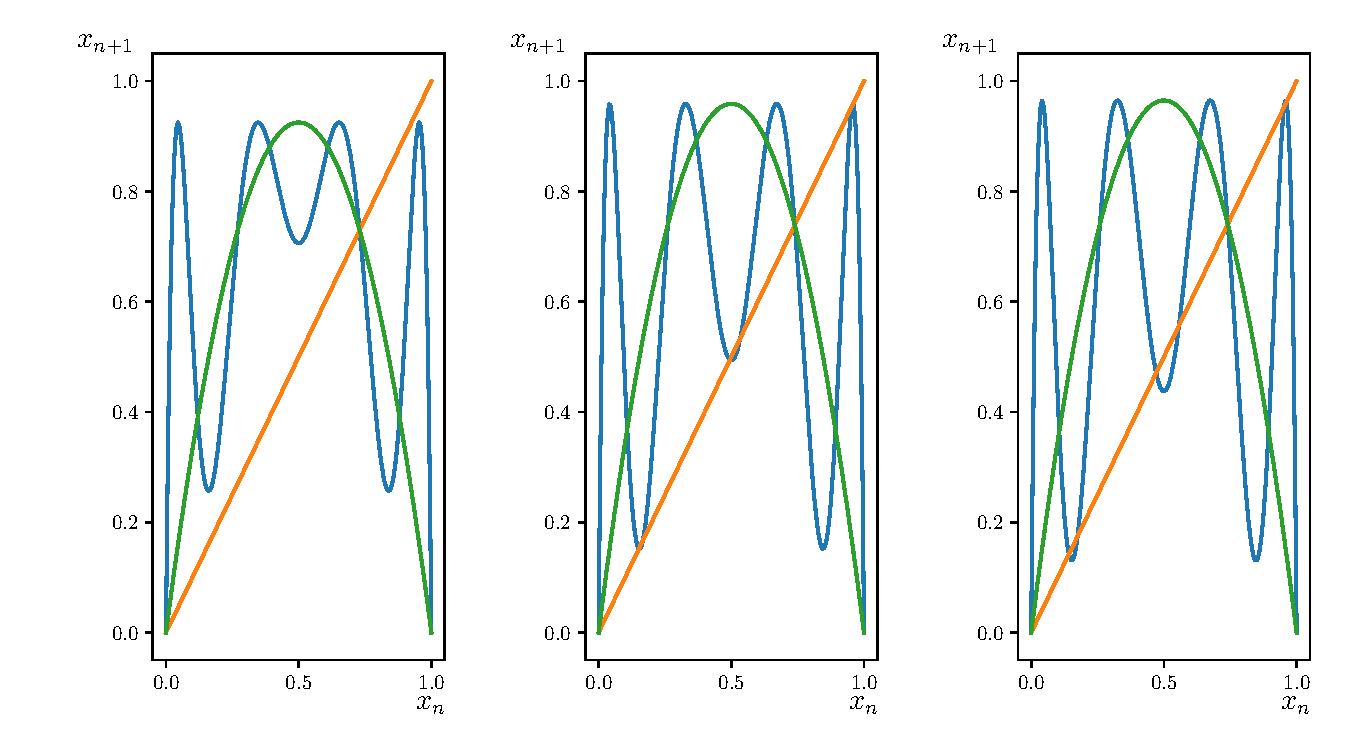
\includegraphics[scale = 0.7]{Figure_5.eps}
	\caption{Comparison of the maps $f$ (green) and $f^3$ (blue) for parameter values $r = 3.7$ (left), $r = 3.835$ (middle)
    and $r = 3.86$ (right). The orange line marks the line $x_{n+1} = x_n$ with intersections indicating a fixed point of the 
    map.}
    \label{fig:comp_log_map}
\end{figure}

\paragraph{}
It is clear that at as $r$ increases from 3.7 to 3.835, a fold bifurcation occurs, with two families of period-3 points appearing. This can be seen both on 
the graphs of the functions themselves (as $r$ increases, $f^3$ crosses the line $x_{n+1} = x_n$ in three 
distinct places, causing six new fixed points of $f^3$ to appear) and in the bifurcation diagram. 
However, the bifurcation diagram seems to suggest that only three of these points are attracting, as 
there are three distinct branches visible in the section of the map where period three orbits are 
obviously discernible. To investigate the stability of these fixed points, we initially sought to 
find the roots of $f^3(x) - x = 0$ analytically, but when this became impossible with our existing 
computing resources we instead sought 
to numerically locate them. 

\paragraph{}
Using Sympy's nsolve command (as this stores results to a higher degree of precision than comparable 
Numpy routines) we sought numerical approximations of the roots, using initial conditions suggested by analysis of 
\autoref{fig:comp_log_map}. This resulted in the following numerical approximations of the 
relevant roots when $r = 3.835$; 0.1520, 0.1672, 0.4945, 0.5340, 0.9543, 0.9586. By computing 
the forward orbits of these points under $f^3$, we were able to show that for each root $a_*$ we have 
$|f^3(a_*) - a_*| < 10^{-15}$. 

\paragraph{}
Next, the value of the derivative was evaluated at these estimated roots. As expected, this 
suggested that one of these families was attracting and one was repelling, with attracting period-3 
points at 0.1520, 0.4945 and at 0.9586. This matches the evidence from the bifurcation diagram 
and provides strong (if not conclusive) support for our hypothesis. Thus we believe that a 
fold bifurcation occurs between $r = 3.7$ and $r = 3.835$, causing two families of 
period-3 points to appear. One of these is attracting and one is repelling (at least near $r = 3.835$). 

\paragraph{}
It is more immediately clear what might be happening when $r = 3.86$. \autoref{fig:bifn_logistic} 
seems to suggest that period-doubling bifurcations occur in the neighborhood of $r = 3.85$. This 
would suggest that the previously attracting family of period-3 points become repelling, so that the 
there are no attracting period-3 points on the other side of the `window' we have previously 
identified.

\section*{Q20}
The bifurcation diagram of the sine map is straightforward to calculate using the same methods 
as in Q16.

\begin{figure}[H]
    \centering
    \hspace{-0.5in}
    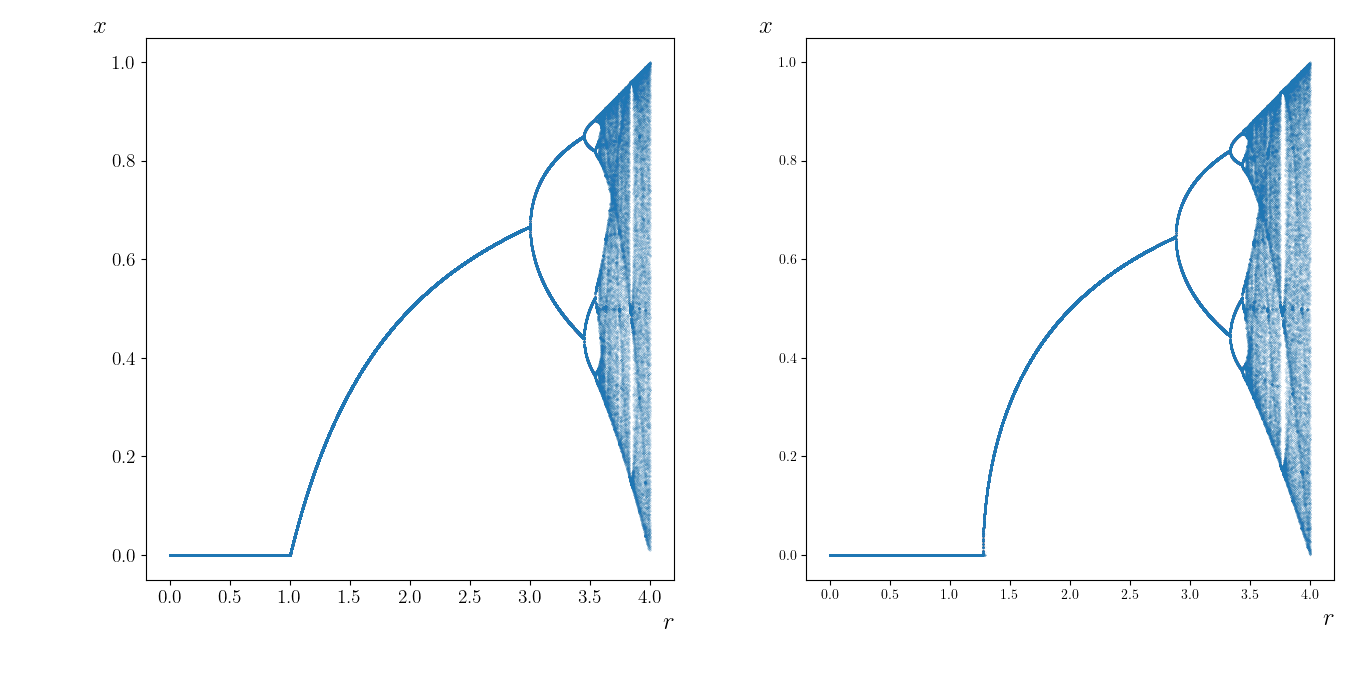
\includegraphics[scale = 0.5]{Figure_6.png}
	\caption{Bifurcation diagrams of the logistic (left) and sine (right) maps.}
    \label{fig:bifn_sin}
\end{figure}

This diagram, while approximate, clearly shows a few features of the system and some marked 
similarities to the bifurcation diagram of the logistic map. Near $r = 0$, the system appears 
to be characterized by a single attracting fixed point at $x = 0$, while for higher values 
at least one other fixed point appears. This makes logical sense, as 
for very low values of $r$ the line $x_{n+1} = x_n$ only intersects the line $x_{n+1} = \frac{r}{4}\sin(\pi x_n)$ 
only once but for higher values it intersects twice (see \autoref{fig:sin_comp_vals}).

\begin{figure}[H]
    \centering
    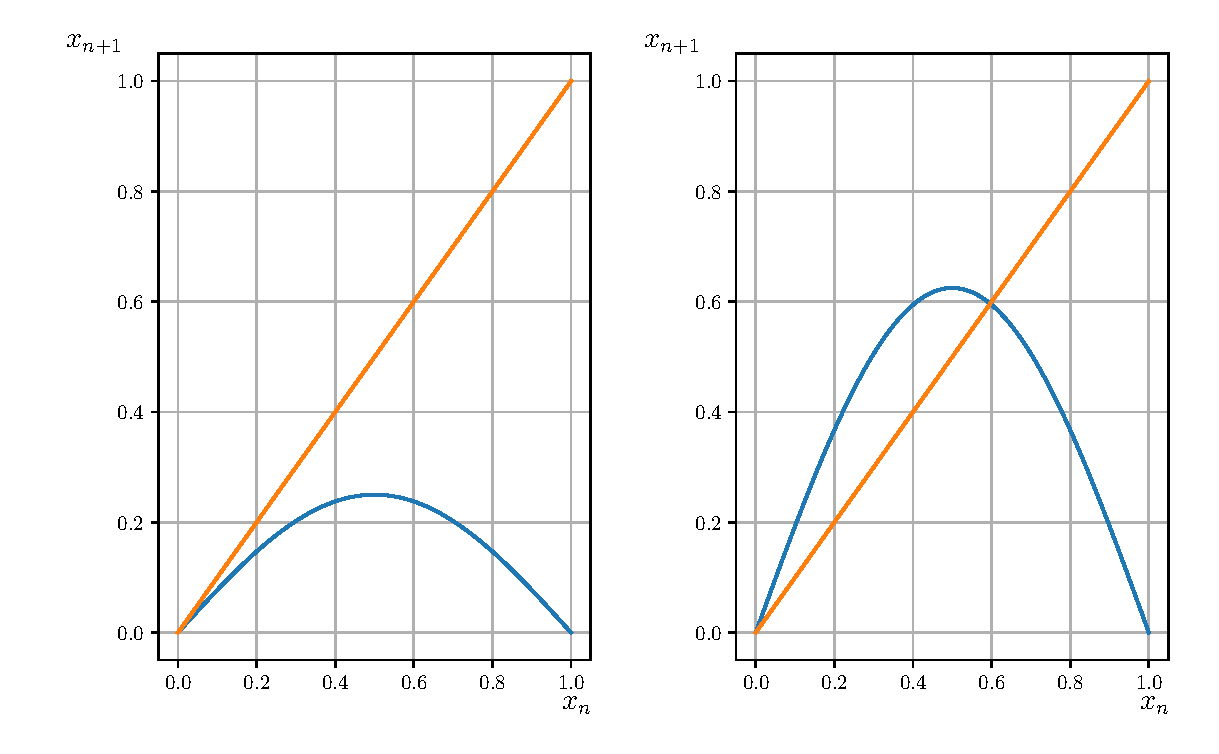
\includegraphics[scale = 0.6]{Figure_7.eps}
	\caption{The Sine Map plotted against $x_{n+1} = x_n$ for low (left, $r = 1$) and high (right, $r = 2.5$) 
    values of $r$.}
    \label{fig:sin_comp_vals}
\end{figure}

\paragraph{}
Since the derivative of $f$ is $f'(x) = 0.25\pi r \cos(\pi x)$ and is thus equal to $0.25\pi r$ at the origin  
it is clear that this fixed point will lose stability when $0.25\pi r \geq 1$ (or, equivalently, 
when $r \geq 4/\pi$). At this parameter value another fixed point will appear as
at the origin $f(0) = 0$, but the slope of $f$ will be greater than the slope of the line 
$x_{n+1} = x_n$. Therefore at least locally $f(x_n) > x_n$ and (since $f$ is continuous and 
$f(1) = 0$) thus another fixed point must appear. This fixed point will be local to the origin 
(see \autoref{fig:sin_comp_vals}) and 
will be attracting (at least for small parameter values). This is because $\cos(x)$ is a decreasing 
function on $[0,\pi/2]$, so if $f'(x) > 1$ at the origin then for a choice of $r$ sufficiently 
close to $4/\pi$ a point near the origin will be such that $|f'| < 1$. 

\paragraph{}
This fixed point appears to remain attracting until approximately $r = 2.75$ where it appears to 
undergo a period-doubling bifurcation and lose stability (see \autoref{fig:sine_map_new} for a sketch 
of behavior on either side of the bifurcation).

\begin{figure}[H]
    \centering
    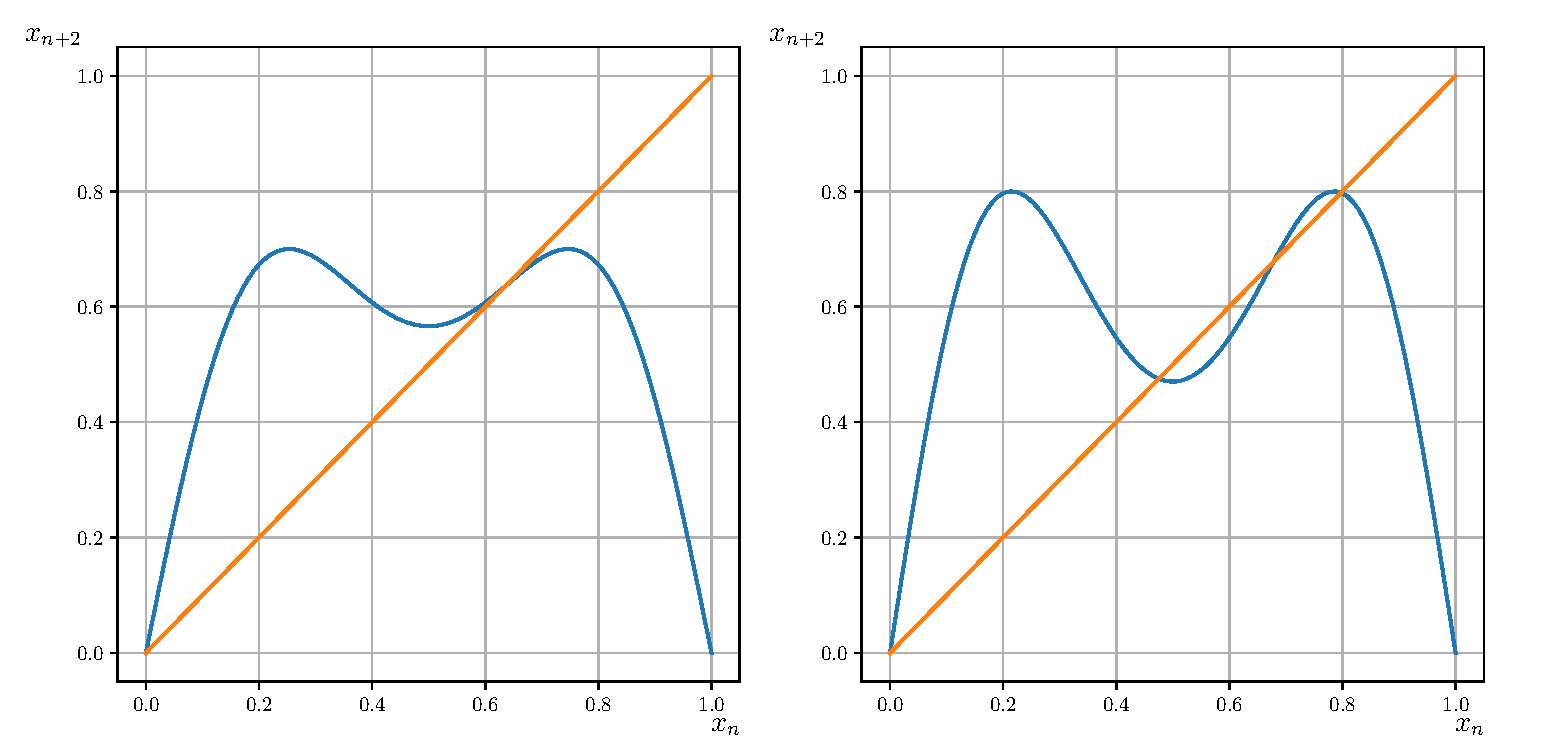
\includegraphics[scale = 0.65]{Figure_Sine_New.eps}
	\caption{Map of $f^2(x_n)$ (blue) and the line $x_{n+2} = x_n$ (orange) on either side of the period doubling 
    bifurcation. From left to 
    right $r = 2.8$, $r= 3.2$.}
    \label{fig:sine_map_new}
\end{figure}

\paragraph{}
These apparent period two orbits also appear 
to be attracting until $r = 3.3$, when they themselves appear to lose stability to another period 
doubling bifurcation. From about $r = 3.5$ 
onwards the system appears to be characterized by complex and chaotic dynamics similar to those 
of the logistic map for higher parameter values (including a `gap' at $r$ close to 3.8). In general, 
the sine and logistic maps appear to display very similar behavior, except that in the sine map 
the parameter at which the fixed point at the origin loses stability is greater than the equivalent 
parameter value for the logistic map. 

\section*{Q21}
\subsection*{(a)}
The maps $T_s$ and $T^2_s$ are straightforward to compute (see \autoref{fig:tent_map_comp} and 
\autoref{fig:tent_map_2_comp})

\begin{figure}[H]
    \centering
    \hspace{-0.50in}
    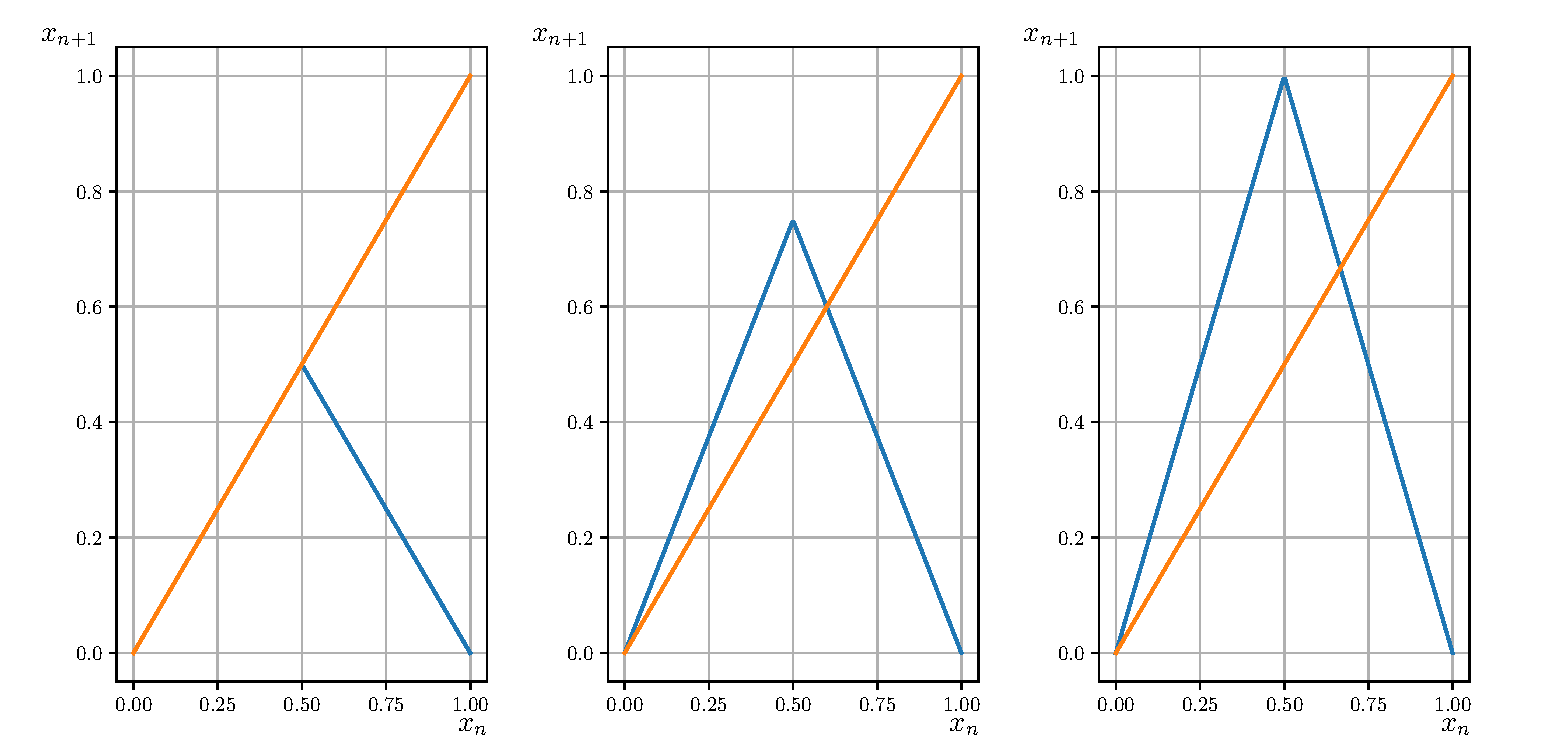
\includegraphics[scale = 0.65]{Figure_8.eps}
	\caption{Map of $T_s$ (blue) and the line $x_{n+1} = x_n$ (orange) for varying values of $s$. From right to 
    left $s = 1$, $s= 1.5$, $s=2$.}
    \label{fig:tent_map_comp}
\end{figure}

\begin{figure}[H]
    \centering
    \hspace{-0.50in}
    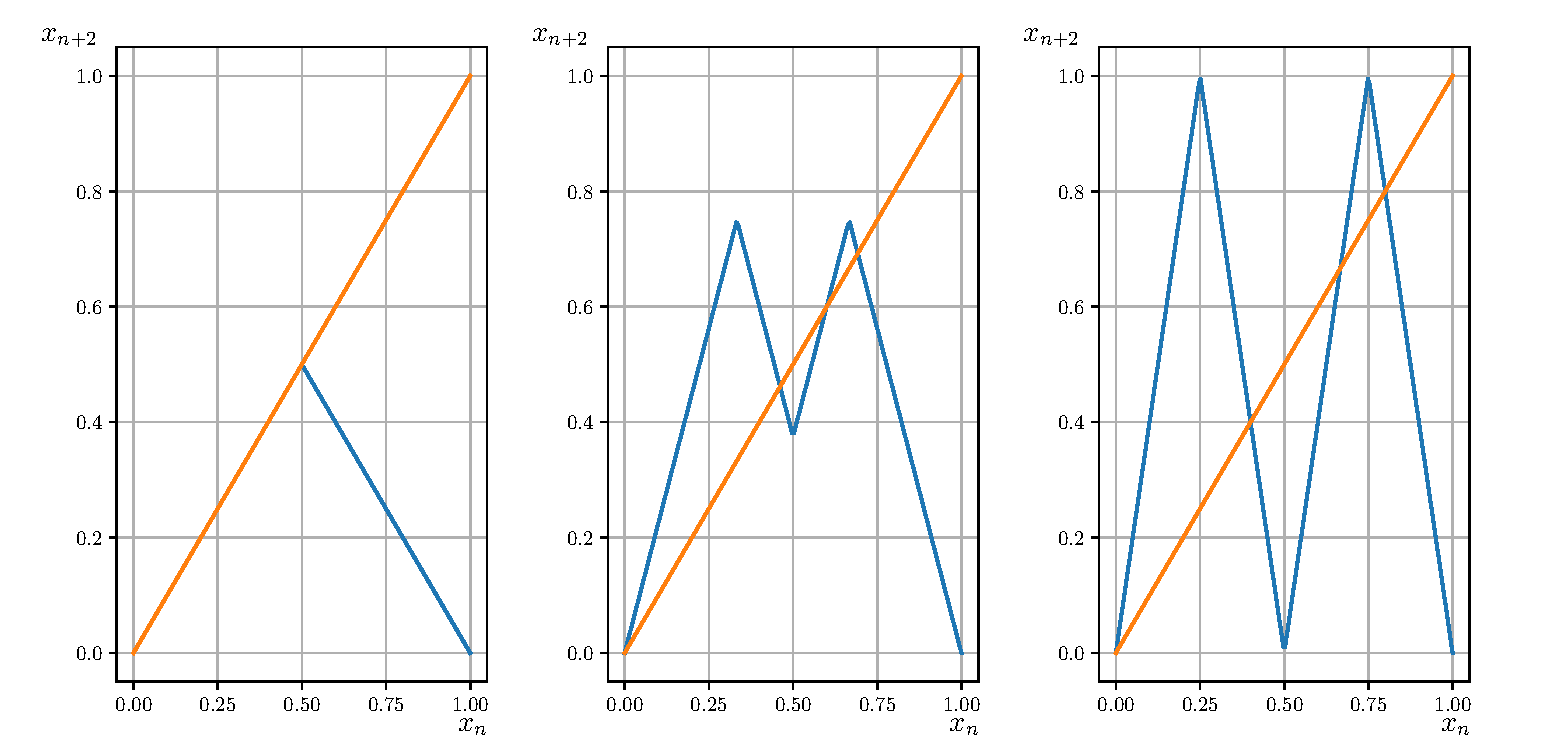
\includegraphics[scale = 0.65]{Figure_9.eps}
	\caption{Map of $T^2_s$ (blue) and the line $x_{n+2} = x_n$ (orange) for varying values of $s$. From right to 
    left $s = 1$, $s= 1.5$, $s=2$.}
    \label{fig:tent_map_2_comp}
\end{figure}



\subsection*{(b)}
\begin{figure}[H]
    \centering
    \hspace{-0.5in}
    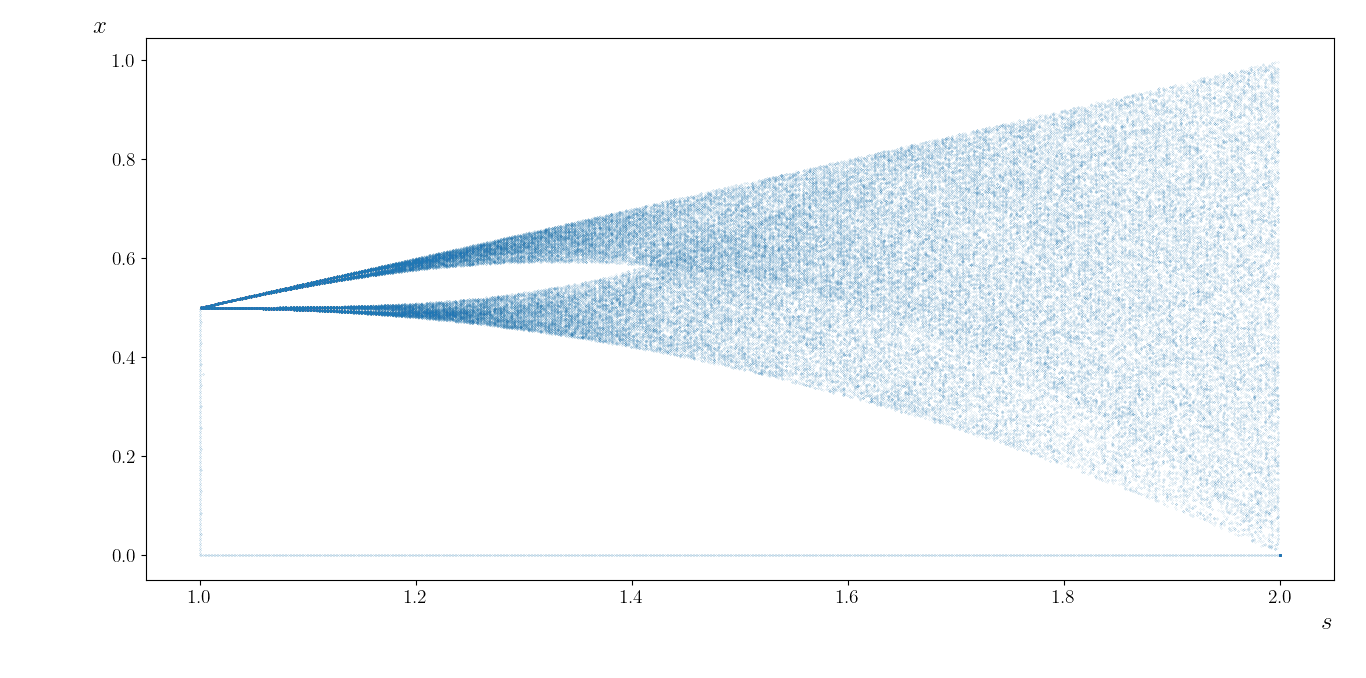
\includegraphics[scale = 0.5]{Figure_10.png}
	\caption{Bifurcation Diagram of the Tent Map from $s = 1$ to $s=2$.}
    \label{fig:bifn_tent}
\end{figure}

\subsection*{(c)}
The bifurcation diagram of the tent map has some superficial similarities to the bifurcation diagrams of the 
logistic and sine maps. However, there are some important differences. At $s =1$ (the minimum 
value we consider) all points in $x \in [0,1/2]$ are fixed under the action of the tent map. None 
of these points are attracting, although they and the fixed point at $x = 1/2$ are Liapunov stable (see below).

\paragraph{}
Considering the fixed points of the tent map in detail, we can see that slope of the map is 
$s$ or $-s$ at any point (except $x = 1/2$). Since $s \in [1,2]$ it follows that no fixed points are attracting in this 
interval (except possibly at points where the function is non-differentiable). This only occurs when 
$s = 1$ ($sx = s(1-x)$ occurs only when $x = 1/2$ and $x = 1/2$ is a fixed point when $s =1$) 
and then for $1/2 > \epsilon > 0$ we have $T(1/2 - \epsilon) = 1/2 - \epsilon = T(1/2 + \epsilon)$ 
so points near $x = 1/2$ do not approach the fixed point. Therefore this point is Liapunov stable 
but not attracting.

\paragraph{}
It is easy to see that for higher order points the slope of $|T^n|$ is $s^n$ except at points where 
$T^n$ is not differentiable. Restricting our analysis to $T^2$ we can express this map as 

\begin{equation*}
    T^2(x) = 
    \begin{cases}
        s^2x & 0 \leq x \leq \frac{1}{2s} \\
        s-s^2x & \frac{1}{2s} \leq x \leq \frac{1}{2} \\
        s-s^2 + s^2x & \frac{1}{2} \leq x \leq 1 - \frac{1}{2s} \\
        s^2-s^2x & 1 - \frac{1}{2s} \leq x \leq 1
    \end{cases}
\end{equation*}

So $T^2$ is not differentiable at $1/2s$, $1/2$ and $1-1/2s$. Clearly when $s=1$ these points are 
equal and we can directly apply our analysis from above (this point is a fixed point and is Liapunov 
stable but not attracting). It remains to show whether any of these points can be elements of a 
period-2 orbit for $s > 1$. Clearly if $s^2x = x$ then $s =1$ (or $x = 0$, but this is a repelling 
fixed point as discussed above) so there are never period-two points 
for $x \in (0,1/2s]$ for $ s> 1$. At $ x = 1/2$ it is straightforward to show that $s- \frac{1}{2}s^2 = \frac{1}{2}$ 
implies that $ s= 1$. Finally if $s^2 - s^2\left(1 - \frac{1}{2s} \right) = \frac{1}{2s}$ then 
by a routine computation this implies that $ s= 1$. Therefore these points are never fixed points of 
$T^2$ for any $s > 1$.

\paragraph{}
In fact, for any 
parameter value between 1 and 2 there are infinitely many periodic orbits, none of which are 
attracting \cite{may_bifn}. From the bifurcation diagram, it appears such orbits are confined 
to two small regions in the domain, although closer inspection reveals that there are in fact 
four such regions (see \autoref{fig:tent_blow_up}).

\begin{figure}[H]
    \centering
    \hspace{-0.5in}
    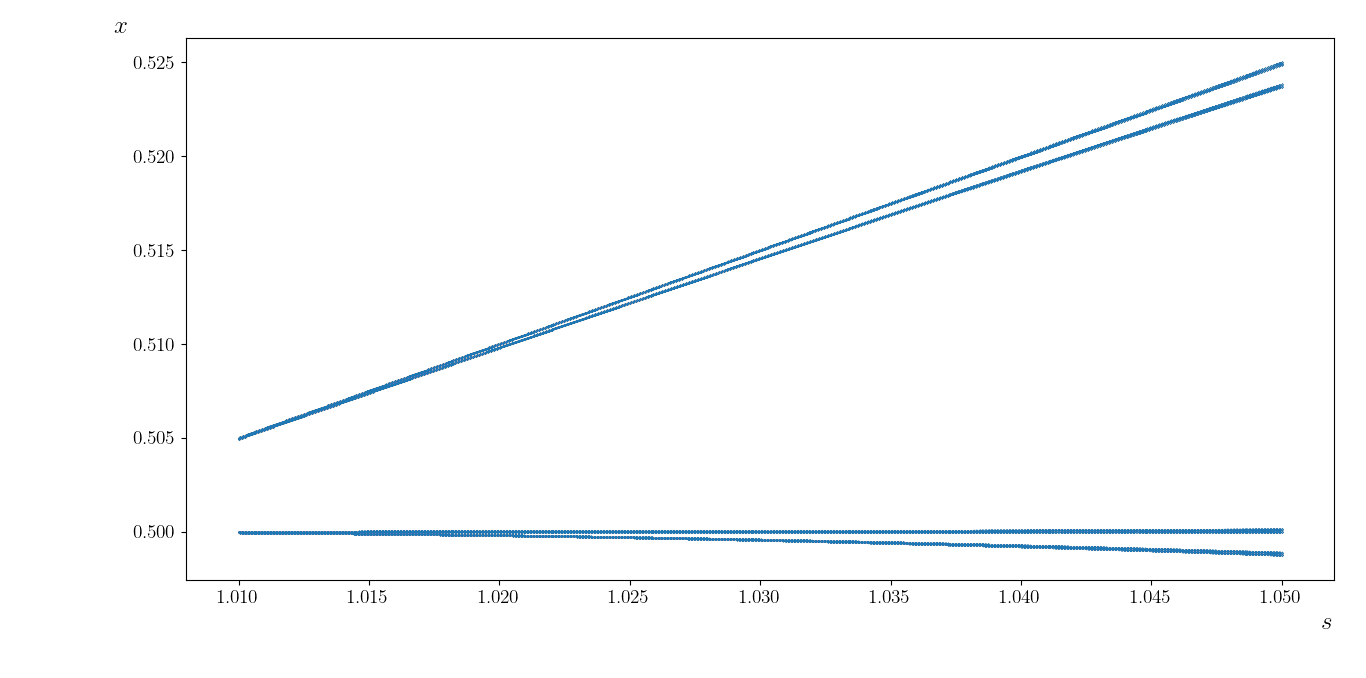
\includegraphics[scale = 0.5]{Figure_Tent_Map_Blowup.png}
	\caption{The bifurcation diagram of the tent map between $s = 1.01$ and $s = 1.05$.}
    \label{fig:tent_blow_up}
\end{figure}

\paragraph{}
However the region in which such behaviors exist grows rapidly as $s$ increases. At approximately 
$s = 2^{1/4}$ two pairs of `arms' appear to merge, forming two larger regions where such orbits 
appear (see \autoref{fig:tent_blow_up_2}). An equivalent merger also appears to occur at $s = 2^{1/2}$ with the remaining two 
arms merging into a single unified region (see \autoref{fig:tent_blow_up_3}).

\begin{figure}[H]
    \centering
    \hspace{-0.5in}
    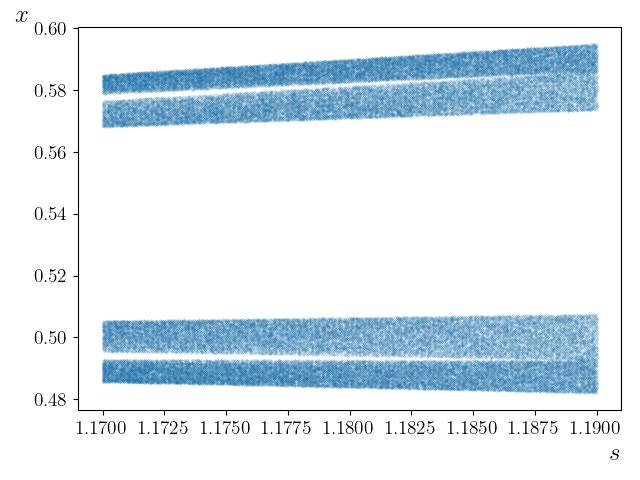
\includegraphics[scale = 0.6]{Figure_Blow_Up_Two.png}
	\caption{The bifurcation diagram of the tent map between $s = 1.17$ and $s = 1.19$.}
    \label{fig:tent_blow_up_2}
\end{figure}

\begin{figure}[H]
    \centering
    \hspace{-0.5in}
    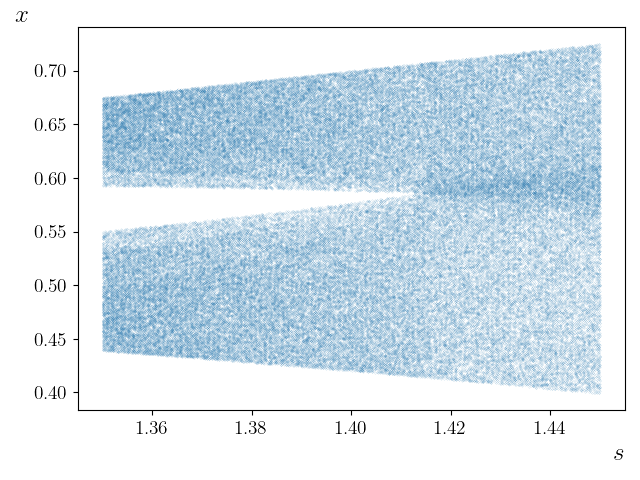
\includegraphics[scale = 0.6]{Figure_Blow_Up_3.png}
	\caption{The bifurcation diagram of the tent map between $s = 1.35$ and $s = 1.45$.}
    \label{fig:tent_blow_up_3}
\end{figure}

\paragraph{}
The exact cause of this behavior is not clear, although it in part reflects the fact that $T^2$ 
maps the area between the two `peaks' in its plot to itself. The discussion in \cite{may_bifn} suggests that 
the point $ s= \sqrt{2}$ is associated with the emergence of the first orbit of an odd period. It is 
also interesting to note that at the point $s = \sqrt{2}$ the map $T^2$ has a slope of two at all differentiable 
points and at the point $s = 2^{1/4}$ the map $T^4$ has a slope of two at all differentiable points. 
This suggests some level of self-similarity between these higher-order iterates of $T$ at these 
points and $T$ at 
$s=2$ although the exact connection is not clear.

\paragraph{}
The exact nature of these dynamics are hard to identify, but it is clear that they share little in 
common with the structure of the logistic or sine maps (at least for smaller values of $s$). Despite 
some superficial similarities in the bifurcation diagram (e.g. what initially appears to be a period-doubling 
bifurcation at $s = 1$) the underlying mechanisms are in fact quite different and produce markedly different results.

\section*{Q1-2021}
\subsection*{(a)}
\begin{figure}[H]
    \centering
    \hspace{-0.5in}
    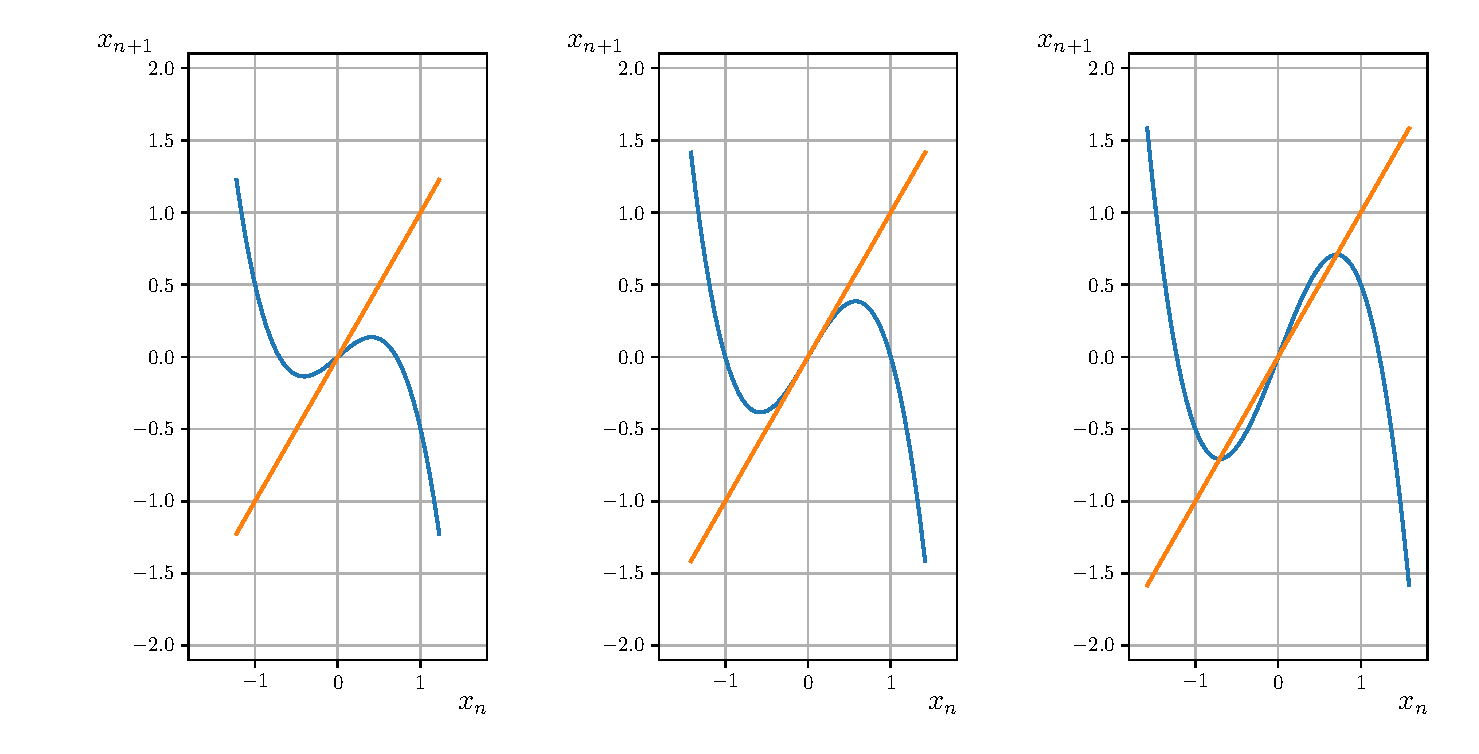
\includegraphics[scale = 0.7]{Figure_11.eps}
	\caption{$f(x)$ (blue) and the line $x_{n+1} = x_n$ (orange) for differing values of $\lambda$. 
    From left to right, $\lambda = 1/2$, $\lambda = 1$ and $\lambda = 3/2$.}
    \label{fig:comp_vals_cubic}
\end{figure}

\subsection*{(b)}
The fixed points of this map are straightforward to find analytically. Setting $f(x) -x = 0$ 
we obtain the polynomial $(\lambda -1)x - x^3 = 0$. This has roots $x = 0$ and $x = \pm \sqrt{\lambda -1}$. 

\subsection*{(c)}
Clearly $f'(x) = \lambda - 3x^2$. If $x = 0$ it is clear that this fixed point is attracting 
when $|\lambda| < 1$. If $x = \pm \sqrt{\lambda -1}$ then this fixed point only exists for $\lambda > 1$ 
and is attracting when $|f'(x)| = |\lambda - 3\lambda +3| = |3 -2\lambda| < 1$. Thus these fixed points 
are attracting for $\lambda \in (1,2)$. 

\subsection*{(d)}
The above suggests a supercritical pitchfork bifurcation occurs at $\lambda = 1$. When $-1 < \lambda < 1$ a single 
attracting fixed point occurs at $x = 0$, but for $1< \lambda < 2$ there are three fixed points. Two of these at 
$x = \pm \sqrt{\lambda -1}$ are attracting and the fixed point at $x = 0$ is repelling.

\subsection*{(e)}
As $\lambda$ increases through $-1$, the fixed point at $x = 0$ gains stability. Furthermore, two 
repelling period-two points appear. Period-two points occur where $f(f(x)) -x = 0$. This is 
equivalent to 

\begin{equation*}
    \lambda(\lambda x - x^3) - (\lambda x - x^3)^3 -x = x(x^2 - (\lambda -1))(x^2 - (\lambda + 1))(x^4 - \lambda x^2 +1) = 0
\end{equation*}

using the hint provided. The roots of this polynomial are at $x = 0$, $x = \pm\sqrt{\lambda -1}$, 
$x = \pm \sqrt{\lambda +1}$ and $x = \pm \sqrt{(\lambda \pm \sqrt{\lambda^2-4})/2}$. Eliminating 
the fixed points (which are not least-period-two points), we can see that at $\lambda = -1$ two 
period-two points emerge (followed by four more at $\lambda = 2$). Then if $x = \pm \sqrt{\lambda +1}$ 
we can find the stability as 

\begin{equation*}
    |f'(\sqrt{\lambda +1})||f'(-\sqrt{\lambda +1})| = |(\lambda - 3\lambda -3)^2| = (-2\lambda -3)^2
\end{equation*}

Clearly $(-2\lambda -3)^2 < 1$ if and only if $|-2\lambda - 3| < 1$ which occurs only when 
$\lambda \in (-2,-1)$, so these period-two points are always repelling (as they only exist for $\lambda > -1$). 

\subsection*{(f)}
As $\lambda$ passes through 2, we know from part (c) that all fixed points become repelling and 
from part (e) that four period-two points appear. This would seem to suggest that these points 
should be repelling, but we this can be confirmed analytically. First, it is useful to note 
that 

\begin{equation}
    f\left(\sqrt{\frac{\lambda - \sqrt{\lambda^2 - 4}}{2}}\right) = \sqrt{\frac{\lambda + \sqrt{\lambda^2 -4}}{2}}
\end{equation}

Since $f$ is odd, the converse is true for $x = -\sqrt{(\lambda -\sqrt{\lambda^2 -4})/2}$. Therefore to 
find the stability of these period-two points, we must find the region where

\begin{align*}
    \left|f'\left(\sqrt{\frac{\lambda - \sqrt{\lambda^2 - 4}}{2}}\right)f\left(\sqrt{\frac{\lambda + \sqrt{\lambda^2 - 4}}{2}}\right)\right| &= \left|\left(\lambda - 3\frac{\lambda - \sqrt{\lambda^2-4}}{2}\right)\left(\lambda - 3\frac{\lambda - \sqrt{\lambda^2-4}}{2}\right)\right| \\
    &= \left|\frac{1}{4}(\lambda + 3\sqrt{\lambda^2 -4})(\lambda - 3\sqrt{\lambda^2 -4}) \right| \\
    &= \left|\frac{1}{4}(\lambda^2 - 9\lambda^2 + 36)\right| \\
    &= |9 - 2\lambda^2| < 1
\end{align*}

This is equivalent to the region where $-1 < 9 - 2\lambda^2 < 1$ or $-10 < -2\lambda^2 < -8$ 
but $\lambda^2 > 0$  so this is simply the region where $4 < \lambda^2 < 5$ so these points are 
attracting for $2 < \lambda < \sqrt{5}$. Therefore at $\lambda = 2$ the two families of period-two points that 
appear are both attracting.

\subsection*{(g)}
See \autoref{fig:bifn_cubic} for the analytically obtained bifurcation diagram (showing fixed points and period-two 
orbits only).

\begin{figure}[H]
    \centering
    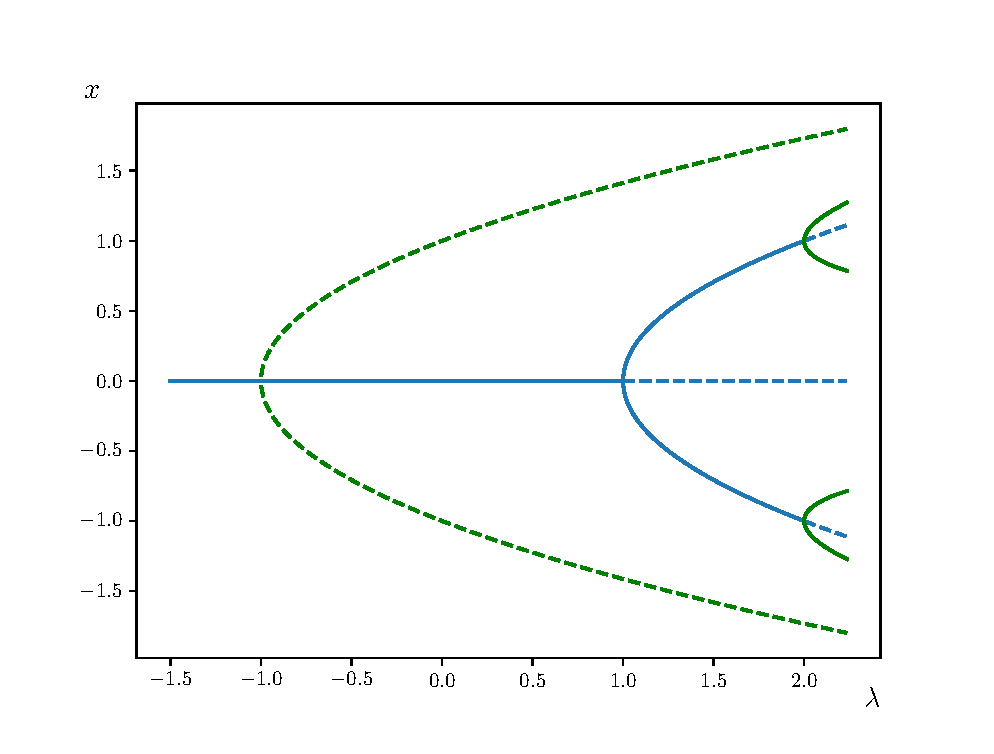
\includegraphics[scale = 0.8]{Figure_12.eps}
	\caption{Analytical bifurcation diagram of the cubic map with fixed points (blue) and 
    period-two orbits (green) only, with attracting points (solid lines) and repelling 
    points (dashed lines) for $\lambda \in [-1,\sqrt{5}]$}.
    \label{fig:bifn_cubic}
\end{figure}

Period doubling bifurcations occur at $\lambda = -1$ and at $\lambda = 2$, while a pitchfork 
bifurcation occurs at $\lambda = 1$. All fixed points become repelling for $\lambda > \sqrt{5}$.

\subsection*{(h)}
While all fixed points we have computed so far lose their stability at $\lambda = \sqrt{5}$, 
other important changes in the dynamics do occur at $\lambda = 3$. To see this, it is useful 
to compute the interior maxima and minima of the cubic map. These critical points occur at the zeros of the 
first derivative of this map, when $\lambda - 3x^2 = 0$ (so $x = \pm \sqrt{\lambda/3}$ at these 
points). The value of the function at these points is 

\begin{equation}
    f(\pm \sqrt{\lambda/3}) = \pm \left(\frac{\lambda^\frac{3}{2}}{3^\frac{1}{2}} - \frac{\lambda^\frac{3}{2}}{3^\frac{3}{2}}\right) = \pm 2\left(\frac{\lambda}{3} \right)^\frac{3}{2} 
\end{equation}

By the hint provided we know that for $\lambda > 3$ the interior maxima and minimas 
exceed $\sqrt{\lambda +1}$ (the converse can also be safely assumed). Therefore, if $\lambda > 3$ 
then for $x_0 = \sqrt{\lambda/3}$ we have $f(x_0) = x_1 > \sqrt{\lambda+1}$. Note that $f(\sqrt{\lambda + 1}) = -\sqrt{\lambda + 1}$ 
and that for all $x \geq \sqrt{\lambda+1}$ we have $f' < -1$. This implies that $f(x_1) < -x_1$. By the oddness of $f$ 
it follows that $f(x_2) = f(f(x_1)) > -f(x_1)$. Therefore this sequence is 
alternating and absolutely diverging (so it contains no convergent subsequence). This is in 
contrast to the case $\lambda < 3$ where points in $[-\sqrt{\lambda +1},\sqrt{\lambda + 1}]$ remained 
inside this set (by the converse of the hint). Therefore all forward orbits of points in this 
interval remained in a compact subset of $\mathbb{R}^2$ and thus contained a convergent subsequence.

\paragraph{}
So at $\lambda = 3$ an important change in the dynamics has occurred. Some points whose forward 
orbits previously 
remained in the set $[-\sqrt{\lambda + 1},\sqrt{\lambda + 1}]$ for all time now escape this set 
and their modulus approaches $\infty$ as $n \rightarrow \infty$.

\section*{Methods}
For the sake of brevity and to avoid unnecessary repetition, we will briefly discuss the methods 
throughout this assignment. Unless shown explicitly in the assignment, computations were performed 
using Python. Analytical computations were performed using Sympy, a Python package for conducting 
algebraic manipulations and simple calculus \cite{sympy}. Numerical methods were implemented using 
Numpy, a library for fast numerical calculations \cite{numpy}. Where possible, bifurcation 
diagrams were obtained analytically, but this was usually not possible (especially where systems are 
characterized by period-doubling bifurcations and/or chaotic behavior). Whether a diagram was 
computed numerically or analytically is noted beneath figure captions. All results are presented 
rounded to four decimal places, but were calculated to at least 16 digits of precision.

\paragraph{}
Numerical bifurcation diagrams were constructed by discretizing the range of possible values for 
the bifurcation parameter and, at each value, computing 1000 iterations of the system on a set of 
initial conditions spaced evenly across the domain of the system. This method is effective at 
detecting stable fixed points (including attracting fixed points, but also points which are Liapunov 
stable may appear if an initial condition sufficiently close to their location is selected), although it will not, in general, detect unstable fixed points. 
For reasons of computational practicality, unstable fixed points are in general not computed. 
Exceptions will be noted where it was possible to obtain fixed points analytically.

\printbibliography
\end{document}